\documentclass[sigconf]{acmart}

\usepackage{booktabs} % For formal tables
\usepackage{graphicx}
\usepackage{rotating}
\definecolor{Gray}{gray}{0.6}


% Copyright
%\setcopyright{none}
%\setcopyright{acmcopyright}
%\setcopyright{acmlicensed}
\setcopyright{rightsretained}
%\setcopyright{usgov}
%\setcopyright{usgovmixed}
%\setcopyright{cagov}
%\setcopyright{cagovmixed}


% DOI
\acmDOI{10.475/123_4}

% ISBN
\acmISBN{123-4567-24-567/08/06}

%Conference
\acmConference[GECCO '17]{the Genetic and Evolutionary Computation Conference 2017}{July 15--19, 2017}{Berlin, Germany}
\acmYear{2017}
\copyrightyear{2017}

\acmPrice{15.00}



%%%%%%%%%%%%%%%%%%%%%%   END OF PREAMBLE   %%%%%%%%%%%%%%%%%%%%%%%%%%%%%%%%%%%%

%%%%%%%%%%%%%%%%%%%%%%%%%%%%%%%%%%%%%%%%%%%%%%%%%%%%%%%%%%%%%%%%%%%%%%%%%%%%%%%
%%%%%%%%% TO BE EDITED %%%%%%%%%%%%%%%%%%%%%%%%%%%%%%%%%%%%%%%%%%%%%%%%%%%%%%%%
%%%%%%%%%%%%%%%%%%%%%%%%%%%%%%%%%%%%%%%%%%%%%%%%%%%%%%%%%%%%%%%%%%%%%%%%%%%%%%%
% rungeneric.py writes data into a subfolder of ppdata
\newcommand{\bbobdatapath}{ppdata/} % change default output folder of COCO if desired
\input{\bbobdatapath cocopp_commands.tex} % provide default of algname and algfolder
% \renewcommand{\algname}{MYNAME}  % name of algorithm as it should appear in the text
% \renewcommand{\algfolder}{ABC/} % subfolder of \bbobdatapath for processed algorithm
%%%%%%%%%%%%%%%%%%%%%%%%%%%%%%%%%%%%%%%%%%%%%%%%%%%%%%%%%%%%%%%%%%%%%%%%%%%%%%%
%%%%%%%%%%%%%%%%%%%%%%%%%%%%%%%%%%%%%%%%%%%%%%%%%%%%%%%%%%%%%%%%%%%%%%%%%%%%%%%
%%%%%%%%%%%%%%%%%%%%%%%%%%%%%%%%%%%%%%%%%%%%%%%%%%%%%%%%%%%%%%%%%%%%%%%%%%%%%%%
\graphicspath{{\bbobdatapath\algfolder}}

\newcommand{\DIM}{\ensuremath{\mathrm{DIM}}}
\newcommand{\aRT}{\ensuremath{\mathrm{aRT}}}
\newcommand{\FEvals}{\ensuremath{\mathrm{FEvals}}}
\newcommand{\nruns}{\ensuremath{\mathrm{Nruns}}}
\newcommand{\Dfb}{\ensuremath{\Delta f_{\mathrm{best}}}}
\newcommand{\Df}{\ensuremath{\Delta f}}
\newcommand{\nbFEs}{\ensuremath{\mathrm{\#FEs}}}
\newcommand{\fopt}{\ensuremath{f_\mathrm{opt}}}
\newcommand{\ftarget}{\ensuremath{f_\mathrm{t}}}
\newcommand{\CrE}{\ensuremath{\mathrm{CrE}}}
\newcommand{\change}[1]{{\color{red} #1}}

\begin{document}


\title{Black-Box Optimization Benchmarking Template for Noiseless Function
Testbed}
\titlenote{Submission deadline: March 31st.}
%Camera-ready paper due April 24th.}}
\subtitle{Draft version}



\author{Firstname Lastname}
%\authornote{tba if needed}
%\orcid{1234-5678-9012}
%\affiliation{%
%  \institution{Institute for Clarity in Documentation}
%  \streetaddress{P.O. Box 1212}
%  \city{Dublin} 
%  \state{Ohio} 
%  \postcode{43017-6221}
%}
%\email{trovato@corporation.com}
%
%\author{G.K.M. Tobin}
%\authornote{The secretary disavows any knowledge of this author's actions.}
%\affiliation{%
%  \institution{Institute for Clarity in Documentation}
%  \streetaddress{P.O. Box 1212}
%  \city{Dublin} 
%  \state{Ohio} 
%  \postcode{43017-6221}
%}
%\email{webmaster@marysville-ohio.com}
%
%\author{Lars Th{\o}rv{\"a}ld}
%\authornote{This author is the
%  one who did all the really hard work.}
%\affiliation{%
%  \institution{The Th{\o}rv{\"a}ld Group}
%  \streetaddress{1 Th{\o}rv{\"a}ld Circle}
%  \city{Hekla} 
%  \country{Iceland}}
%\email{larst@affiliation.org}
%
%\author{Lawrence P. Leipuner}
%\affiliation{
%  \institution{Brookhaven Laboratories}
%  \streetaddress{P.O. Box 5000}}
%\email{lleipuner@researchlabs.org}
%
%\author{Sean Fogarty}
%\affiliation{%
%  \institution{NASA Ames Research Center}
%  \city{Moffett Field}
%  \state{California} 
%  \postcode{94035}}
%\email{fogartys@amesres.org}
%
%\author{Charles Palmer}
%\affiliation{%
%  \institution{Palmer Research Laboratories}
%  \streetaddress{8600 Datapoint Drive}
%  \city{San Antonio}
%  \state{Texas} 
%  \postcode{78229}}
%\email{cpalmer@prl.com}
%
%\author{John Smith}
%\affiliation{\institution{The Th{\o}rv{\"a}ld Group}}
%\email{jsmith@affiliation.org}
%
%\author{Julius P.~Kumquat}
%\affiliation{\institution{The Kumquat Consortium}}
%\email{jpkumquat@consortium.net}

% The default list of authors is too long for headers}
\renewcommand{\shortauthors}{Firstname Lastname et. al.}


\begin{abstract}
to be written
\end{abstract}


%
% The code below should be generated by the tool at
% http://dl.acm.org/ccs.cfm
% Please copy and paste the code instead of the example below. 
%
 \begin{CCSXML}
<ccs2012>
<concept>
<concept_id>10010147.10010178.10010205.10010208</concept_id>
<concept_desc>Computing methodologies~Continuous space search</concept_desc>
<concept_significance>500</concept_significance>
</concept>
</ccs2012>
\end{CCSXML}

\ccsdesc[500]{Computing methodologies~Continuous space search}


% We no longer use \terms command
%\terms{Algorithms}

% Complete with anything that is needed
\keywords{Benchmarking, Black-box optimization}

\maketitle


% \section{Introduction}
%
% \section{Algorithm Presentation}
%
% \section{Experimental Procedure}
% \subsection{Parameter Tuning}
%
%%%%%%%%%%%%%%%%%%%%%%%%%%%%%%%%%%%%%%%%%%%%%%%%%%%%%%%%%%%%%%%%%%%%%%%%%%%%%%%
\section{CPU Timing}
%%%%%%%%%%%%%%%%%%%%%%%%%%%%%%%%%%%%%%%%%%%%%%%%%%%%%%%%%%%%%%%%%%%%%%%%%%%%%%%
% note that the following text is just a proposal and can/should be changed to your needs:
In order to evaluate the CPU timing of the algorithm, we have run the \change{MY-ALGORITHM-NAME} on the  \change{bbob test suite \cite{hansen2009fun}} with restarts for a maximum budget equal to \change{$400 (D + 2)$} function evaluations according to \cite{hansen2016exp}. The \change{C/Java/Python/Matlab/Octave} code was run on a \change{Mac Intel(R) Core(TM) i5-2400S CPU @ 2.50GHz} with \change{1} processor and \change{4} cores \change{and (compile) options xxx}. The time per function evaluation for dimensions 2, 3, 5, 10, 20\change{, 40} equals \change{$x.x$}, \change{$x.x$}, \change{$x.x$}, \change{$xx$}, \change{$xxx$}\change{, and $xxx$} seconds respectively. 


%%%%%%%%%%%%%%%%%%%%%%%%%%%%%%%%%%%%%%%%%%%%%%%%%%%%%%%%%%%%%%%%%%%%%%%%%%%%%%%
\section{Results}
%%%%%%%%%%%%%%%%%%%%%%%%%%%%%%%%%%%%%%%%%%%%%%%%%%%%%%%%%%%%%%%%%%%%%%%%%%%%%%%

Results of \algname\ from experiments according to \cite{hansen2016exp} and \cite{hansen2016perfass} on the benchmark
functions given in \cite{wp200901_2010,hansen2012fun} are presented in
Figures~\ref{fig:aRTgraphs}, \ref{fig:RLDs}, \ref{tab:aRTloss}, and \ref{fig:aRTlogloss} and in
Tables~\ref{tab:aRTs}. The experiments were performed with COCO \cite{hansen2016cocoplat}, version \change{2.0}, the plots were produced with version \change{2.0}.


%%%%%%%%%%%%%%%%%%%%%%%%%%%%%%%%%%%%%%%%%%%%%%%%%%%%%%%%%%%%%%%%%%%%%%%%%%%%%%%
%%%%%%%%%%%%%%%%%%%%%%%%%%%%%%%%%%%%%%%%%%%%%%%%%%%%%%%%%%%%%%%%%%%%%%%%%%%%%%%

% Scaling of aRT with dimension

%%%%%%%%%%%%%%%%%%%%%%%%%%%%%%%%%%%%%%%%%%%%%%%%%%%%%%%%%%%%%%%%%%%%%%%%%%%%%%%
\begin{figure*}
\begin{tabular}{l@{\hspace*{-0.0\textwidth}}l@{\hspace*{-0.0\textwidth}}l@{\hspace*{-0.0\textwidth}}l}
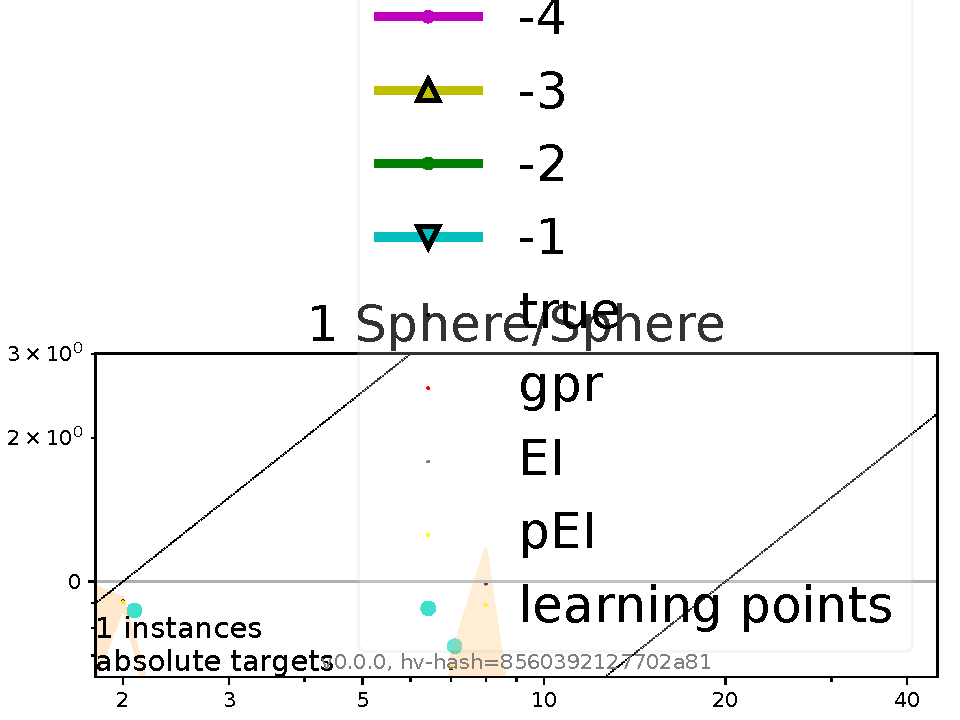
\includegraphics[width=0.24\textwidth]{ppfigdim_f001}&
\includegraphics[width=0.24\textwidth]{ppfigdim_f002}&
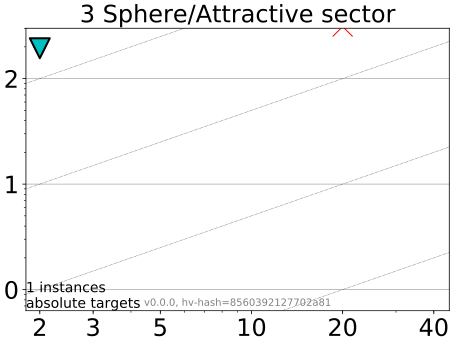
\includegraphics[width=0.24\textwidth]{ppfigdim_f003}&
\includegraphics[width=0.24\textwidth]{ppfigdim_f004}\\[-1ex]
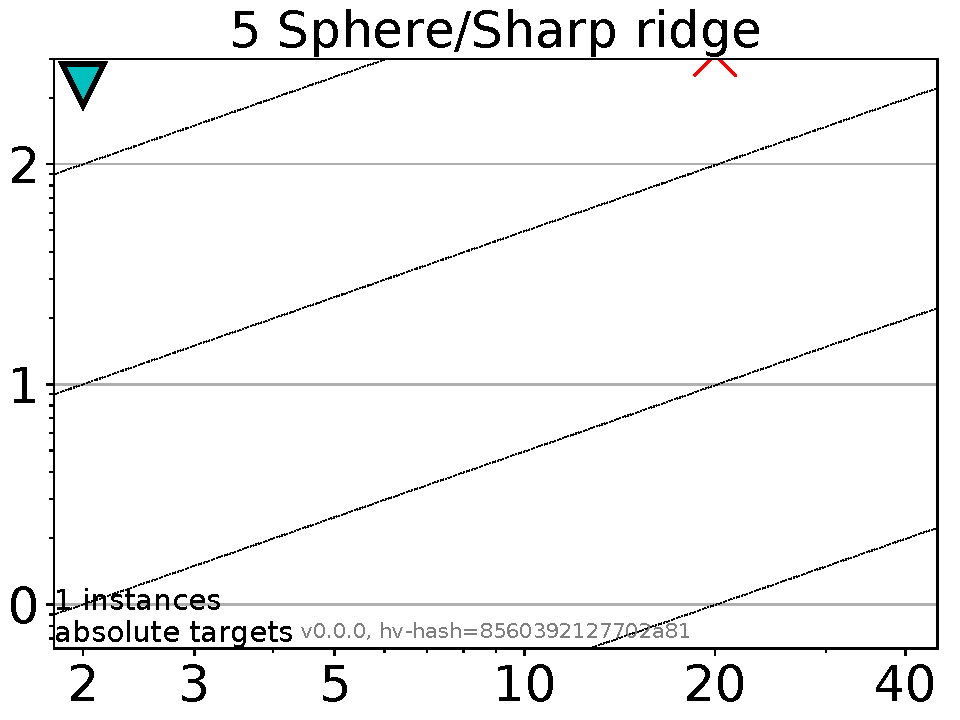
\includegraphics[width=0.24\textwidth]{ppfigdim_f005}&
\includegraphics[width=0.24\textwidth]{ppfigdim_f006}&
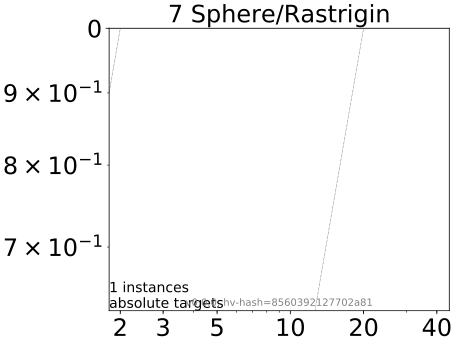
\includegraphics[width=0.24\textwidth]{ppfigdim_f007}&
\includegraphics[width=0.24\textwidth]{ppfigdim_f008}\\[-1ex]
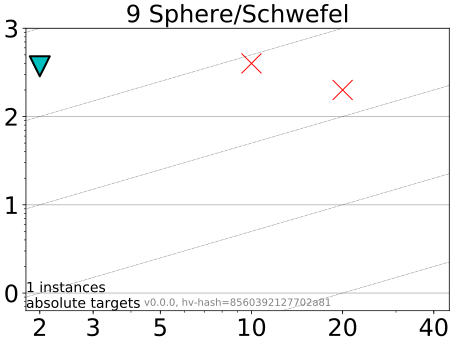
\includegraphics[width=0.24\textwidth]{ppfigdim_f009}&
\includegraphics[width=0.24\textwidth]{ppfigdim_f010}&
\includegraphics[width=0.24\textwidth]{ppfigdim_f011}&
\includegraphics[width=0.24\textwidth]{ppfigdim_f012}\\[-1ex]
\includegraphics[width=0.24\textwidth]{ppfigdim_f013}&
\includegraphics[width=0.24\textwidth]{ppfigdim_f014}&
\includegraphics[width=0.24\textwidth]{ppfigdim_f015}&
\includegraphics[width=0.24\textwidth]{ppfigdim_f016}\\[-1ex]
\includegraphics[width=0.24\textwidth]{ppfigdim_f017}&
\includegraphics[width=0.24\textwidth]{ppfigdim_f018}&
\includegraphics[width=0.24\textwidth]{ppfigdim_f019}&
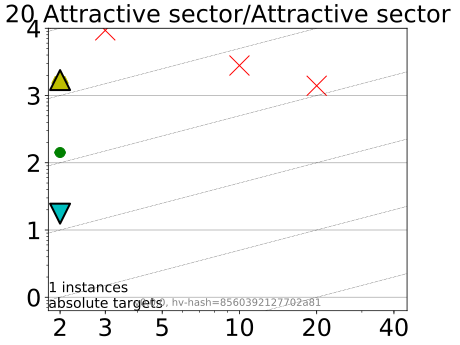
\includegraphics[width=0.24\textwidth]{ppfigdim_f020}\\[-1ex]
\includegraphics[width=0.24\textwidth]{ppfigdim_f021}&
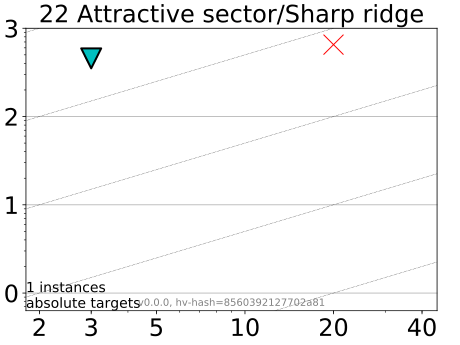
\includegraphics[width=0.24\textwidth]{ppfigdim_f022}&
\includegraphics[width=0.24\textwidth]{ppfigdim_f023}&
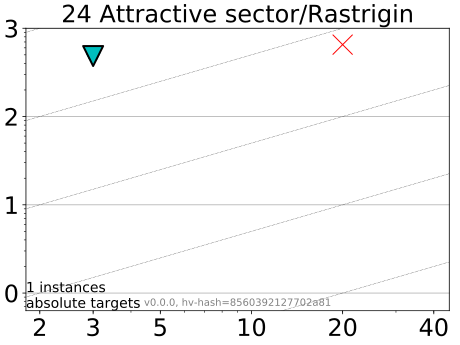
\includegraphics[width=0.24\textwidth]{ppfigdim_f024}
\end{tabular}
\vspace{-3ex}
 \caption{\label{fig:aRTgraphs}
 \bbobppfigdimlegend{$f_1$ and $f_{24}$}
 }
\end{figure*}

%%%%%%%%%%%%%%%%%%%%%%%%%%%%%%%%%%%%%%%%%%%%%%%%%%%%%%%%%%%%%%%%%%%%%%%%%%%%%%%
%%%%%%%%%%%%%%%%%%%%%%%%%%%%%%%%%%%%%%%%%%%%%%%%%%%%%%%%%%%%%%%%%%%%%%%%%%%%%%%
 
% Table showing the average runtime (aRT in number of function
% evaluations) divided by the best aRT measured during BBOB-2009 (given in the
% first row of each cell) for functions $f_1$--$f_{24} for dimension 5$.

%%%%%%%%%%%%%%%%%%%%%%%%%%%%%%%%%%%%%%%%%%%%%%%%%%%%%%%%%%%%%%%%%%%%%%%%%%%%%%%

\begin{table*}\tiny
%\hfill5-D\hfill~\\[1ex]
{\normalsize \color{red}
\ifthenelse{\isundefined{\algorithmG}}{}{more than 6 algorithms: please split the tables below by hand until it fits to the page limits}
}
\mbox{\begin{minipage}[t]{0.499\textwidth}\tiny
\centering
\pptableheader 

\input{\bbobdatapath\algfolder pptable_f001_05D} 

\input{\bbobdatapath\algfolder pptable_f002_05D}

\input{\bbobdatapath\algfolder pptable_f003_05D}

\input{\bbobdatapath\algfolder pptable_f004_05D}

\input{\bbobdatapath\algfolder pptable_f005_05D}

\input{\bbobdatapath\algfolder pptable_f006_05D}

\input{\bbobdatapath\algfolder pptable_f007_05D}

\input{\bbobdatapath\algfolder pptable_f008_05D}

\input{\bbobdatapath\algfolder pptable_f009_05D}

\input{\bbobdatapath\algfolder pptable_f010_05D}

\input{\bbobdatapath\algfolder pptable_f011_05D}

\input{\bbobdatapath\algfolder pptable_f012_05D}

\pptablefooter

\end{minipage}
\hspace{0.002\textwidth}
\begin{minipage}[t]{0.499\textwidth}\tiny
\centering

\pptableheader 

\input{\bbobdatapath\algfolder pptable_f013_05D}

\input{\bbobdatapath\algfolder pptable_f014_05D}

\input{\bbobdatapath\algfolder pptable_f015_05D}

\input{\bbobdatapath\algfolder pptable_f016_05D}

\input{\bbobdatapath\algfolder pptable_f017_05D}

\input{\bbobdatapath\algfolder pptable_f018_05D}

\input{\bbobdatapath\algfolder pptable_f019_05D}

\input{\bbobdatapath\algfolder pptable_f020_05D}

\input{\bbobdatapath\algfolder pptable_f021_05D}

\input{\bbobdatapath\algfolder pptable_f022_05D}

\input{\bbobdatapath\algfolder pptable_f023_05D}

\input{\bbobdatapath\algfolder pptable_f024_05D}

\pptablefooter

\end{minipage}}

\caption[Table of aRTs]{\label{tab:aRTs5}\bbobpptablecaption{dimension $5$}
}
\end{table*}


%%%%%%%%%%%%%%%%%%%%%%%%%%%%%%%%%%%%%%%%%%%%%%%%%%%%%%%%%%%%%%%%%%%%%%%%%%%%%%%
%%%%%%%%%%%%%%%%%%%%%%%%%%%%%%%%%%%%%%%%%%%%%%%%%%%%%%%%%%%%%%%%%%%%%%%%%%%%%%%

% Table showing the average runtime (aRT in number of function
% evaluations) divided by the best aRT measured during BBOB-2009 (given in the
% first row of each cell) for functions $f_1$--$f_{24} for dimension 20$.

%%%%%%%%%%%%%%%%%%%%%%%%%%%%%%%%%%%%%%%%%%%%%%%%%%%%%%%%%%%%%%%%%%%%%%%%%%%%%%%
\begin{table*}\tiny
%\hfill20-D\hfill~\\[1ex]
\mbox{\begin{minipage}[t]{0.499\textwidth}\tiny
\centering
\pptableheader 

\input{\bbobdatapath\algfolder pptable_f001_20D} 

\input{\bbobdatapath\algfolder pptable_f002_20D}

\input{\bbobdatapath\algfolder pptable_f003_20D}

\input{\bbobdatapath\algfolder pptable_f004_20D}

\input{\bbobdatapath\algfolder pptable_f005_20D}

\input{\bbobdatapath\algfolder pptable_f006_20D}

\input{\bbobdatapath\algfolder pptable_f007_20D}

\input{\bbobdatapath\algfolder pptable_f008_20D}

\input{\bbobdatapath\algfolder pptable_f009_20D}

\input{\bbobdatapath\algfolder pptable_f010_20D}

\input{\bbobdatapath\algfolder pptable_f011_20D}

\input{\bbobdatapath\algfolder pptable_f012_20D}

\pptablefooter

\end{minipage}
\hspace{0.002\textwidth}
\begin{minipage}[t]{0.499\textwidth}\tiny
\centering
\pptableheader 

\input{\bbobdatapath\algfolder pptable_f013_20D}

\input{\bbobdatapath\algfolder pptable_f014_20D}

\input{\bbobdatapath\algfolder pptable_f015_20D}

\input{\bbobdatapath\algfolder pptable_f016_20D}

\input{\bbobdatapath\algfolder pptable_f017_20D}

\input{\bbobdatapath\algfolder pptable_f018_20D}

\input{\bbobdatapath\algfolder pptable_f019_20D}

\input{\bbobdatapath\algfolder pptable_f020_20D}

\input{\bbobdatapath\algfolder pptable_f021_20D}

\input{\bbobdatapath\algfolder pptable_f022_20D}

\input{\bbobdatapath\algfolder pptable_f023_20D}

\input{\bbobdatapath\algfolder pptable_f024_20D}

\pptablefooter

\end{minipage}}
 
\caption[Table of aRTs]{\label{tab:aRTs20}\bbobpptablecaption{dimension $20$}
}
\end{table*}

%%%%%%%%%%%%%%%%%%%%%%%%%%%%%%%%%%%%%%%%%%%%%%%%%%%%%%%%%%%%%%%%%%%%%%%%%%%%%%%


%%%%%%%%%%%%%%%%%%%%%%%%%%%%%%%%%%%%%%%%%%%%%%%%%%%%%%%%%%%%%%%%%%%%%%%%%%%%%%%
%%%%%%%%%%%%%%%%%%%%%%%%%%%%%%%%%%%%%%%%%%%%%%%%%%%%%%%%%%%%%%%%%%%%%%%%%%%%%%%

% Empirical cumulative distribution functions (ECDFs) per function group.

%%%%%%%%%%%%%%%%%%%%%%%%%%%%%%%%%%%%%%%%%%%%%%%%%%%%%%%%%%%%%%%%%%%%%%%%%%%%%%%
\newcommand{\rot}[2][2.5]{
  \hspace*{-3.5\baselineskip}%
  \begin{rotate}{90}\hspace*{#1em}#2\vspace{0.5em}
  \end{rotate}}
\begin{figure*}
\begin{tabular}{l@{\hspace*{-0.00\textwidth}}l@{\hspace*{0.01\textwidth}}|l@{\hspace*{-0.00\textwidth}}l}
\multicolumn{2}{c}{$D=5$} & \multicolumn{2}{c}{$D=20$}\\[-0.5ex]
\rot[3]{all functions}
\includegraphics[width=0.2362\textwidth]{pprldistr_05D_noiselessall} &
\includegraphics[width=0.2362\textwidth]{ppfvdistr_05D_noiselessall} &
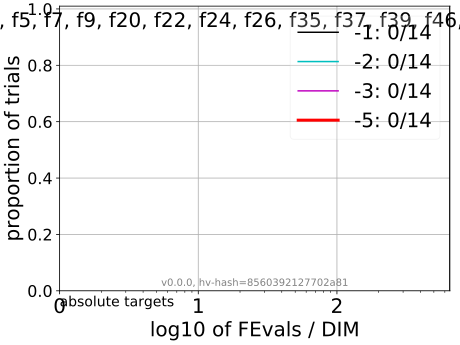
\includegraphics[width=0.2362\textwidth]{pprldistr_20D_noiselessall} &
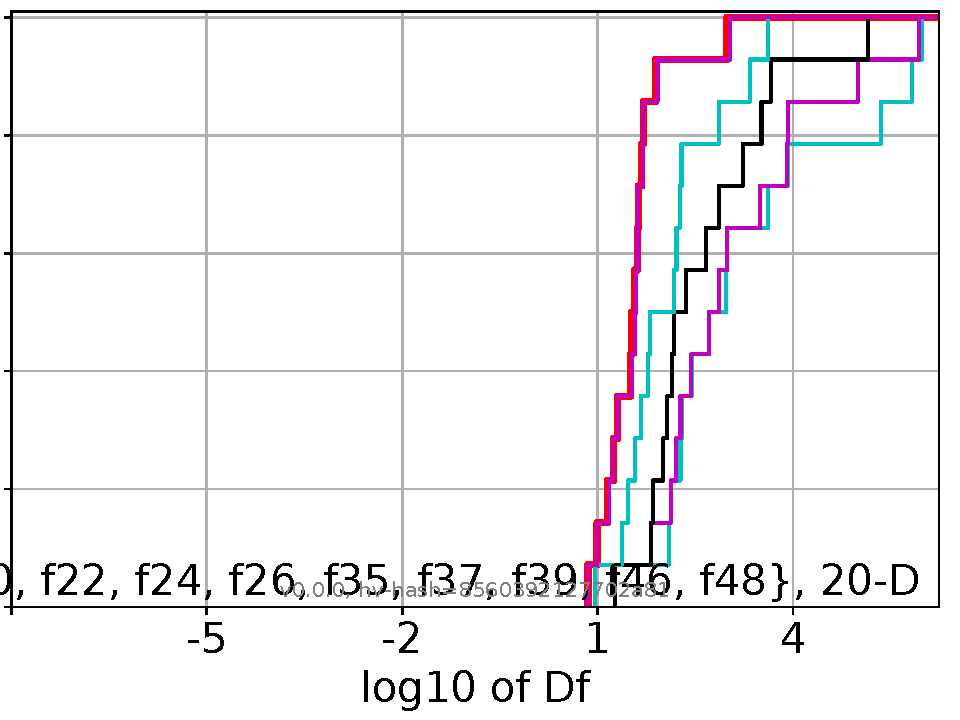
\includegraphics[width=0.2362\textwidth]{ppfvdistr_20D_noiselessall} \\[-0.2em]
\rot[2.9]{separable fcts}
\includegraphics[width=0.2362\textwidth]{pprldistr_05D_separ} &
\includegraphics[width=0.2362\textwidth]{ppfvdistr_05D_separ} &
\includegraphics[width=0.2362\textwidth]{pprldistr_20D_separ} &
\includegraphics[width=0.2362\textwidth]{ppfvdistr_20D_separ} \\[-0.2em]
\rot[1.45]{misc.\ moderate fcts}
\includegraphics[width=0.2362\textwidth]{pprldistr_05D_lcond} &
\includegraphics[width=0.2362\textwidth]{ppfvdistr_05D_lcond} &
\includegraphics[width=0.2362\textwidth]{pprldistr_20D_lcond} &
\includegraphics[width=0.2362\textwidth]{ppfvdistr_20D_lcond} \\[-0.2em]
\rot[1.5]{ill-conditioned fcts}
\includegraphics[width=0.2362\textwidth]{pprldistr_05D_hcond} &
\includegraphics[width=0.2362\textwidth]{ppfvdistr_05D_hcond} &
\includegraphics[width=0.2362\textwidth]{pprldistr_20D_hcond} &
\includegraphics[width=0.2362\textwidth]{ppfvdistr_20D_hcond} \\[-0.2em]
\rot[2.3]{multi-modal fcts}
\includegraphics[width=0.2362\textwidth]{pprldistr_05D_multi} &
\includegraphics[width=0.2362\textwidth]{ppfvdistr_05D_multi} &
\includegraphics[width=0.2362\textwidth]{pprldistr_20D_multi} &
\includegraphics[width=0.2362\textwidth]{ppfvdistr_20D_multi} \\[-0.2em]
\rot[1.7]{weak structure fcts}
\includegraphics[width=0.2362\textwidth]{pprldistr_05D_mult2} &
\includegraphics[width=0.2362\textwidth]{ppfvdistr_05D_mult2} &
\includegraphics[width=0.2362\textwidth]{pprldistr_20D_mult2} &
\includegraphics[width=0.2362\textwidth]{ppfvdistr_20D_mult2}
\vspace*{-1ex}
\end{tabular}
 \caption{\label{fig:RLDs}
 \bbobpprldistrlegend{}
 }
\end{figure*}
%%%%%%%%%%%%%%%%%%%%%%%%%%%%%%%%%%%%%%%%%%%%%%%%%%%%%%%%%%%%%%%%%%%%%%%%%%%%%%%


%%%%%%%%%%%%%%%%%%%%%%%%%%%%%%%%%%%%%%%%%%%%%%%%%%%%%%%%%%%%%%%%%%%%%%%%%%%%%%%
%%%%%%%%%%%%%%%%%%%%%%%%%%%%%%%%%%%%%%%%%%%%%%%%%%%%%%%%%%%%%%%%%%%%%%%%%%%%%%%

% aRT loss ratios (figure and table)

%%%%%%%%%%%%%%%%%%%%%%%%%%%%%%%%%%%%%%%%%%%%%%%%%%%%%%%%%%%%%%%%%%%%%%%%%%%%%%%
\begin{figure}
\centering
\parbox{0.48\columnwidth}{\centering 5-D}\hfill
\parbox{0.48\columnwidth}{\centering 20-D}\\
\includegraphics[width=0.48\columnwidth]{pplogloss_05D_noiselessall}\hfill
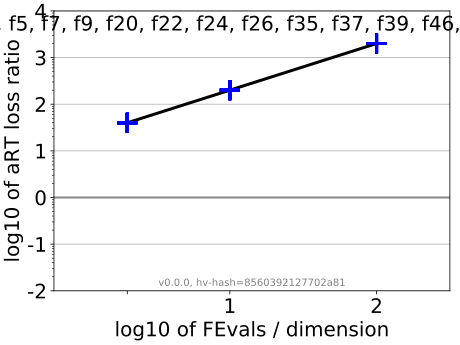
\includegraphics[width=0.48\columnwidth]{pplogloss_20D_noiselessall}\\[2ex]
%
\input{\bbobdatapath\algfolder pploglosstable_05D_noiselessall}\\
\input{\bbobdatapath\algfolder pploglosstable_20D_noiselessall}
\caption{\label{tab:aRTloss}%
\bbobloglosstablecaption{}
}
\end{figure}


%%%%%%%%%%%%%%%%%%%%%%%%%%%%%%%%%%%%%%%%%%%%%%%%%%%%%%%%%%%%%%%%%%%%%%%%%%%%%%%
%%%%%%%%%%%%%%%%%%%%%%%%%%%%%%%%%%%%%%%%%%%%%%%%%%%%%%%%%%%%%%%%%%%%%%%%%%%%%%%

% aRT loss ratios per function group

%%%%%%%%%%%%%%%%%%%%%%%%%%%%%%%%%%%%%%%%%%%%%%%%%%%%%%%%%%%%%%%%%%%%%%%%%%%%%%%
\begin{figure}
\begin{tabular}{@{}l@{}@{}l@{}}
\multicolumn{1}{c}{5-D} & \multicolumn{1}{c}{20-D}\\
%\rot{all functions}
%\hspace*{-2mm}
\rot[2.8]{separable fcts}
\hspace*{-1.4mm}
\includegraphics[width=0.24\textwidth]{pplogloss_05D_separ} &
\includegraphics[width=0.24\textwidth]{pplogloss_20D_separ}\\
\rot[2.7]{moderate fcts}
\hspace*{-1.4mm}
\includegraphics[width=0.24\textwidth]{pplogloss_05D_lcond} &
\includegraphics[width=0.24\textwidth]{pplogloss_20D_lcond}\\
\rot[1.9]{ill-conditioned fcts}
\hspace*{-1.35mm}
\includegraphics[width=0.24\textwidth]{pplogloss_05D_hcond} &
\includegraphics[width=0.24\textwidth]{pplogloss_20D_hcond}\\
\rot[2.5]{multi-modal fcts}
\hspace*{-1.3mm}
\includegraphics[width=0.24\textwidth]{pplogloss_05D_multi} &
\includegraphics[width=0.24\textwidth]{pplogloss_20D_multi}\\
\rot[1.6]{weak structure fcts}
\hspace*{-1.4mm}
\includegraphics[width=0.24\textwidth]{pplogloss_05D_mult2} &
\includegraphics[width=0.24\textwidth]{pplogloss_20D_mult2}
\vspace*{-0.5ex}
\end{tabular}
 \caption{\label{fig:aRTlogloss}%
\bbobloglossfigurecaption{}
}
\end{figure}

%%%%%%%%%%%%%%%%%%%%%%%%%%%%%%%%%%%%%%%%%%%%%%%%%%%%%%%%%%%%%%%%%%%%%%%%%%%%%%%


%%%%%%%%%%%%%%%%%%%%%%%%%%%%%%%%%%%%%%%%%%%%%%%%%%%%%%%%%%%%%%%%%%%%%%%%%%%%%%%
%\section{Discussion}  % and or conclusion, summary...
%%%%%%%%%%%%%%%%%%%%%%%%%%%%%%%%%%%%%%%%%%%%%%%%%%%%%%%%%%%%%%%%%%%%%%%%%%%%%%%

\bibliographystyle{ACM-Reference-Format}
\bibliography{bbob}  % bbob.bib is the name of the Bibliography in this case

\clearpage % otherwise the last figure might be missing

\end{document}